\documentclass[a4paper]{article}
\usepackage{amsmath,amssymb,caption,enumitem,float,geometry,graphicx,indentfirst,minted,parskip,tabularx,xcolor}
\usepackage{booktabs}
\captionsetup[figure]{labelsep=period}
\definecolor{bg}{rgb}{0.95,0.95,0.95}
\geometry{left=3.5cm,right=3.5cm,top=3.3cm,bottom=3.3cm}
\setlength{\parindent}{2em}
\usemintedstyle{emacs}
\begin{document}
\begin{titlepage}
    \vspace*{0.25cm}
    \noindent\rule[0.25\baselineskip]{\textwidth}{1pt}
    \begin{center}
        \huge{\textsc{UM--SJTU Joint Institute}}\vspace{0.3em}\\
        \huge{\textbf{Embedded System Design (VE373)}}\vspace{0.3em}\\
        \Large{(Design of Microprocessor Based Systems)}
        \noindent\rule[0.25\baselineskip]{\textwidth}{1pt}
    \end{center}
    \begin{center}
        \vspace{5cm}
        \Large{\textsc{Project Proposal}}\vspace{0.5em}\\
        \Large{\textbf{Hexapod Spider}}\vspace{1em}\\
        \Large{\textbf{Group 8}}\\
    \end{center}
    \vfill
    \large
    \begin{tabular}{ll}
        Name: Yihua Liu \hspace*{2em}&ID: 518021910998\hspace*{2em}\\
        Name: Xingyuan Wang \hspace*{2em}&ID: 518370910198\hspace*{2em}\\
        Name: Haorong Lu \hspace*{2em}&ID: 518370910194\hspace*{2em}\\
        \\
        Date: \today
    \end{tabular}
\end{titlepage}
\tableofcontents
\newpage
\section{Objectives}
\begin{itemize}
    \item Implement a simple hexapod robot with multiple movement postures.
    \item Control the robot remotely with hand gestures.
    \item Implement auto collision avoiding and LED state display if time allows.
\end{itemize}
\section{Overview}
In this project, we design and implement a hexapod robot which can be controlled remotely using gestures. The robot uses 6 feet to move, and has the basic functions including restoring posture, moving forward, moving backward, turning clockwise, and turning counterclockwise. The movement of the robot is controlled by hand gestures using a wearable device via Bluetooth. Two PIC32 boards are used in the project, with one controlling the movement of the robot spider, and the other detecting and sending gesture control signals to the robot.
\section{Mechanical Structure Diagram}
\begin{figure}[H]
    \centering
    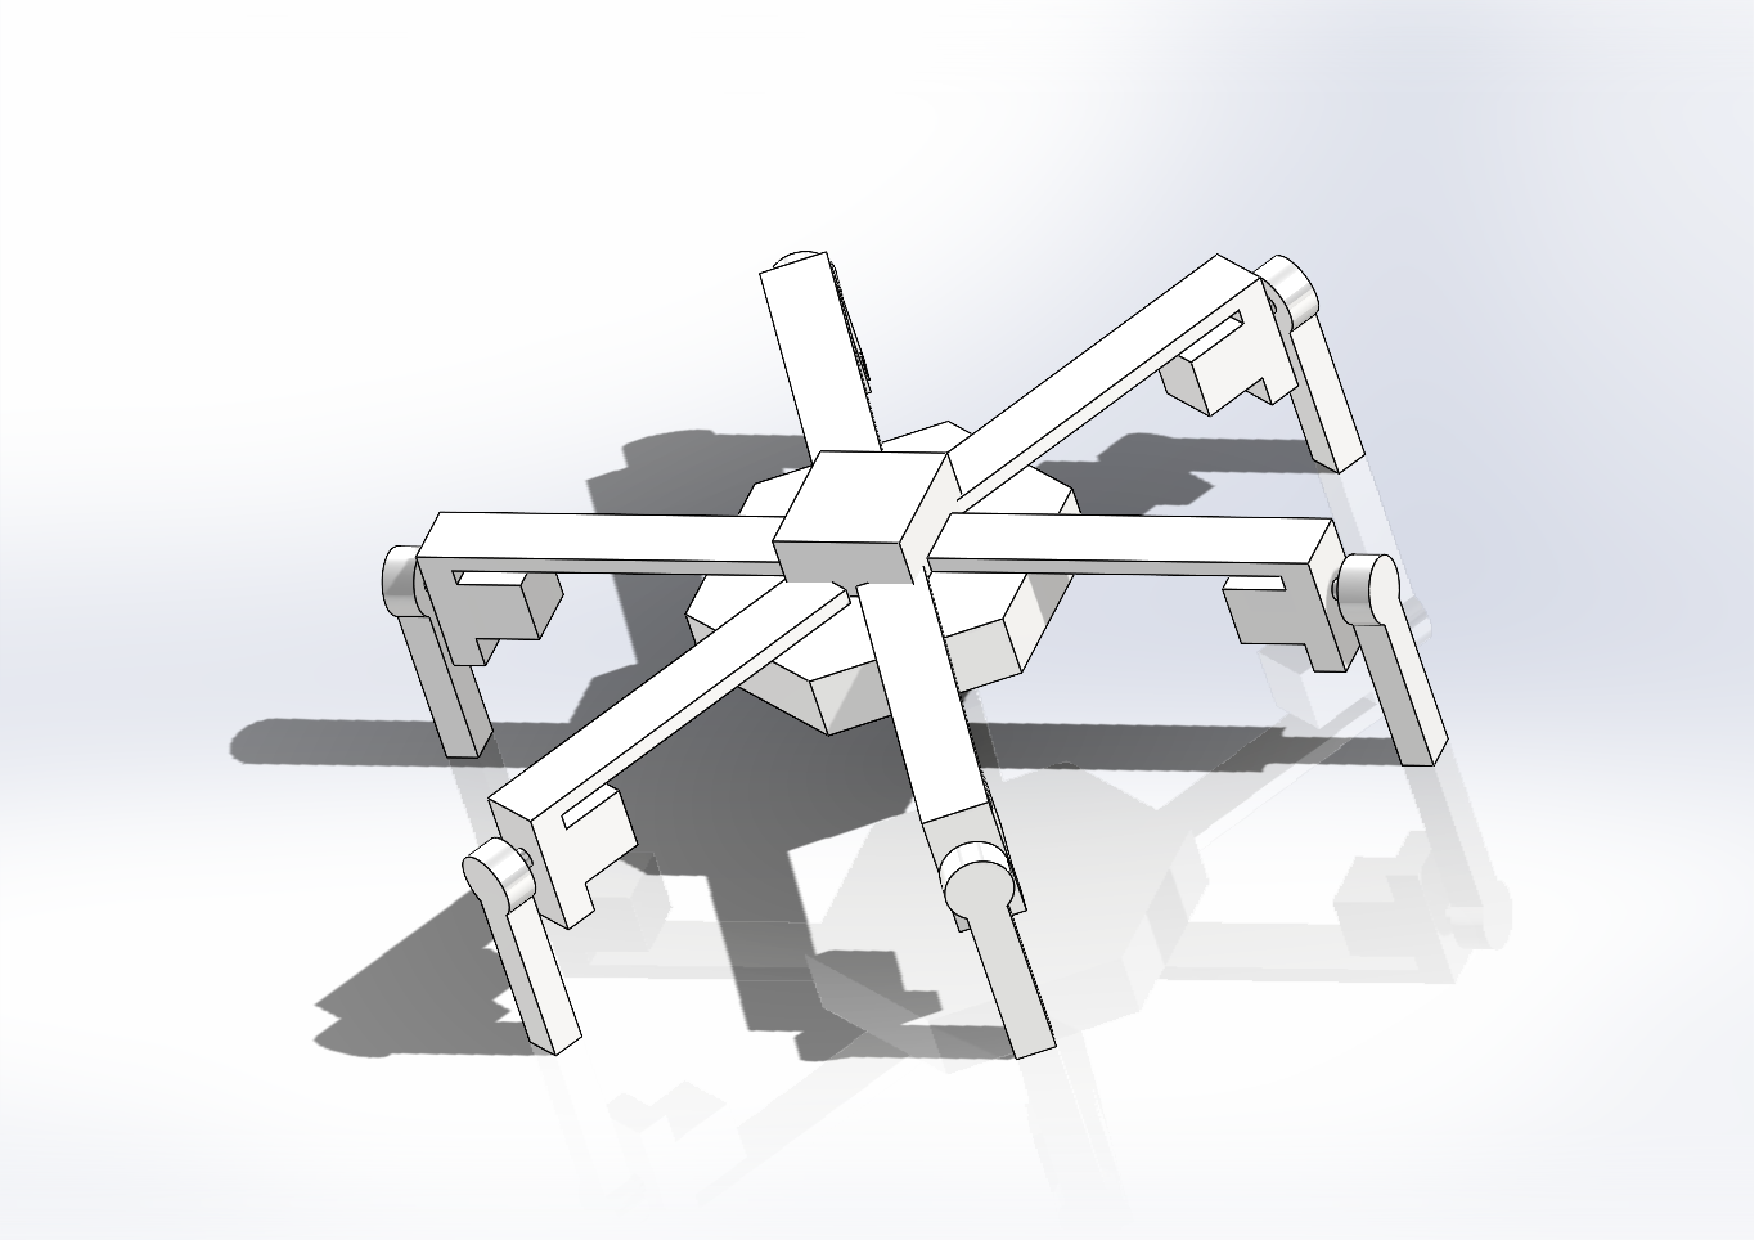
\includegraphics[width=1\textwidth]{Mechanical_Structure_2D.pdf}
    \caption{Component diagram of MPU-6050.}
\end{figure}
\section{Functional Block Diagram}
\begin{figure}[H]
    \centering
    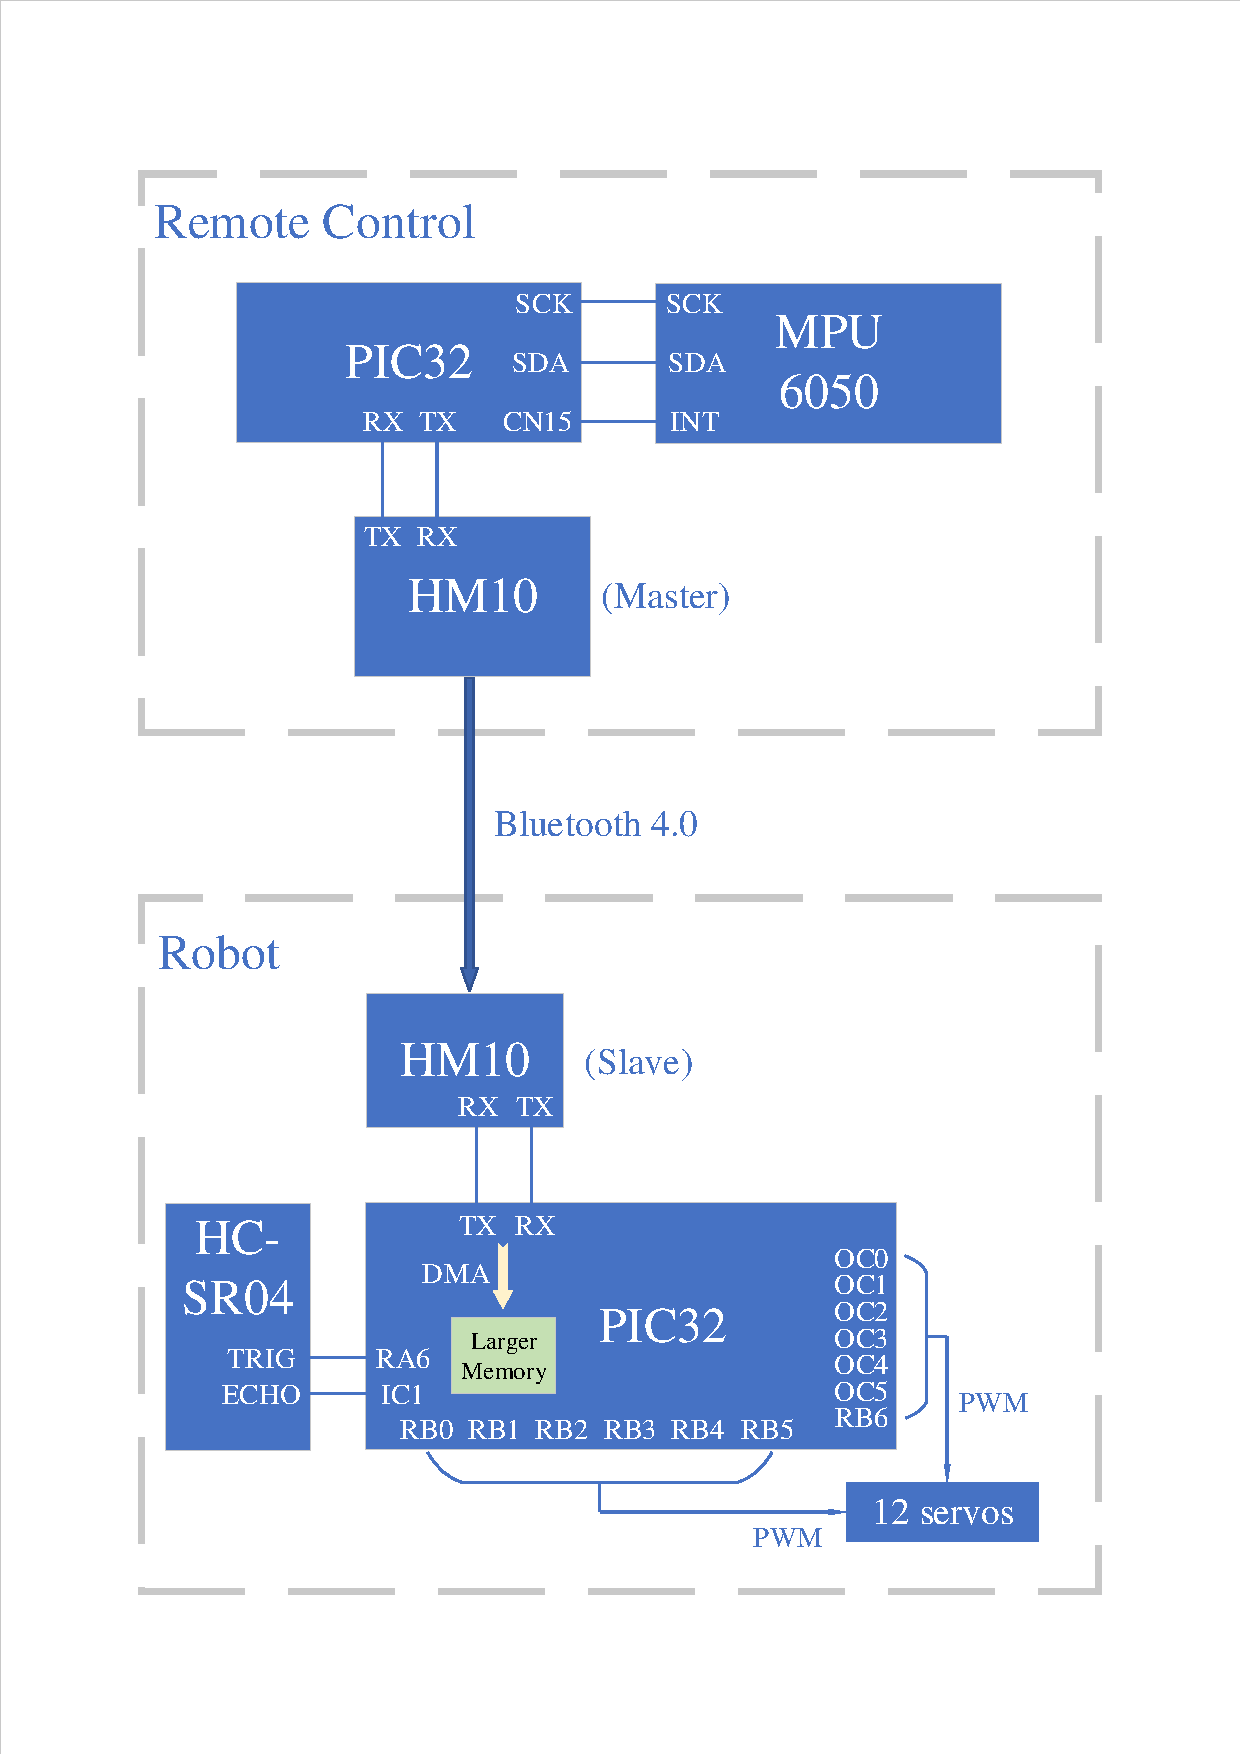
\includegraphics[width=1\textwidth]{Diagram.pdf}
    \caption{Functional Block Diagram.}
\end{figure}

\section{Component Diagram}
This section covers the main peripheral components used in our project.
\subsection{Motion Tracking Device}
In this project, we use MPU-6050, which is an six DoF accelerometer and gyroscope as our motion tracking device for remote control using hands. It measures temperature, acceleration and gravity data in x, y and z axis directions, and communicates with our microprocessor using I2C protocol. The pins used in our program have been labelled in the following diagram.
\begin{figure}[H]
    \centering
    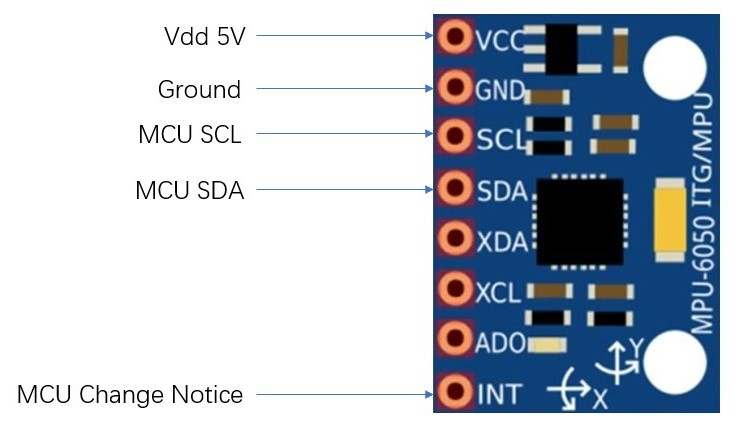
\includegraphics[width=1\textwidth]{MPU.jpg}
    \caption{Component diagram of MPU-6050.}
\end{figure}
VCC pin is connected to power supply for MPU-6050, and GND pin is connected to the same ground as PIC32. SCL and SDA are the pins to be connected with I2C ports of PIC32. We note that the MPU operates in a slave mode while the MCU operates in the master mode. MPU-6050 supports 400kHz fast mode I2C and programmable interrupts which can be checked through INT pin. In our case, we only enable data-available interrupt and connect it to the change notice pin (CN15) of our MCU. The other three pins are for auxiliary data and clock, and address transportation, which are not needed in our case.
\subsection{Bluetooth Module}
We choose HM-10 Bluetooth module in our project to establish the remote connection between control side and conduct side. Currently we are only considering using the Bluetooth module on the control side as transmitter and using the module on the conduct side as receiver, with motion instructions being transmitted. Bidirectional communication might be implemented in the future.
\begin{figure}[H]
    \centering
    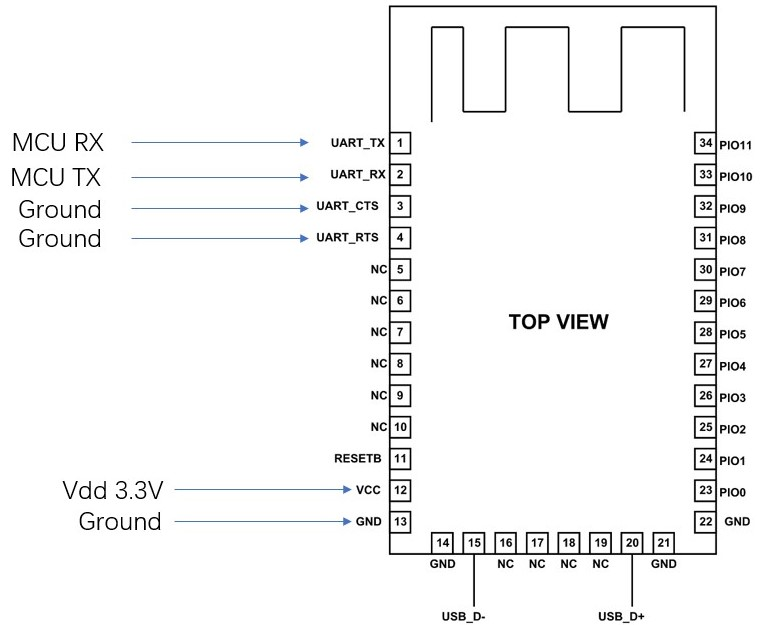
\includegraphics[width=1\textwidth]{HM10.jpg}
    \caption{Component diagram of HM-10.}
\end{figure}
As only the fundamental data transmission mode is used in our project, only 6 pins labelled in the diagram is needed. The Bluetooth module is connected to our PIC32 via UART with a required baud rate being 9600. On the control side, the Bluetooth is configured to be in master mode so that it will search for the other Bluetooth module which is in the slave mode. Bluetooth module setup is done by sending instruction strings via the UART TX pin on the MCU to the Bluetooth module before communication is established.

On the receiving side, DMA will be be used to transmit received data to a larger space as soon as the receiver has data available.

\subsection{Servo}
In this project, we use 12 servo motors to control the motion of the 6 legs of our spider, since each leg needs to move upward, downward, forward and backward. We choose MG90S as our servo, which has a rotating angle between 0 and 180 degrees controlled by PWM signals. The required frequency of the PWM signal is 50Hz. The following diagram shows the pinout of the servo.

\begin{figure}[H]
    \centering
    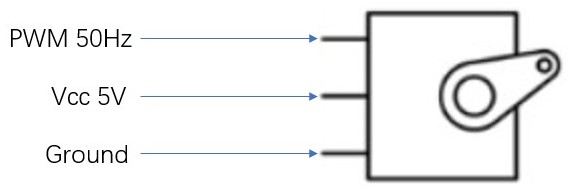
\includegraphics[width=0.7\textwidth]{servo.jpg}
    \caption{Component diagram of MG90S.}
\end{figure}

As can be seen from the diagram, we need one PWM signal per servo which make a total of 12 PWM signals. Unfortunately, PIC32 does not have that many output compare modules. Therefore, we intend to use up all available output compare modules and use GPIO with the timer and interrupt to make up for the shortage.

\subsection{Distance Detector}
We plan to add an ultrasonic distance sensor HC-SR04 on our spider facing forward which detects the distance between the spider and potential obstruction in its front. The diagram of HC-SR04 is shown below.
\begin{figure}[H]
    \centering
    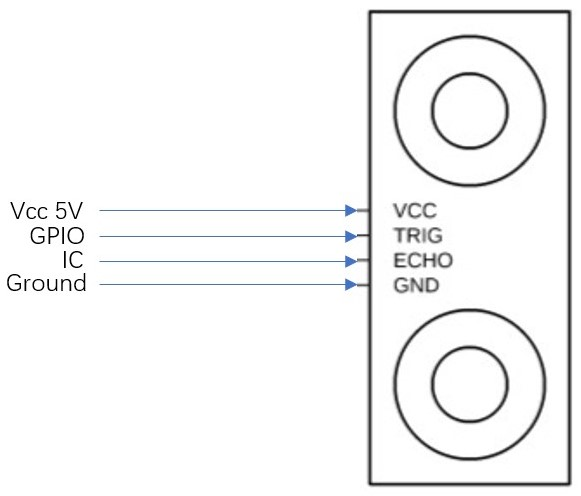
\includegraphics[width=0.5\textwidth]{SR.jpg}
    \caption{Component diagram of HC-SR04.}
\end{figure}
The GPIO pin of PIC32 connected to TRIG pin in HC-SR04 sends a high value exceeding 10$\mu s$ to trigger the distance measurement. If any signal comes back to the module, the distance will be proportional to time of high value on ECHO pin. In this case, we use an input capture module to measure that time of high value on ECHO pin. When the distance is below a certain value, the spider is expected to refuse moving forward.

\section{Preliminary Component List}

\begin{table}[htbp]
    \centering
    \begin{tabular}{ccc}    
        \toprule    
            Part & Part Number & Price (rmb) \\    
        \midrule
            PIC32 Board   (x2)     & PIC32MX795F512L      & N/A    \\
            Accelerometer          & MPU6050 6DOF         & 14     \\
            Bluetooth   Tx/Rx      & HM-10                & 42     \\
            Arduino Motor   Shield & REV3                 & 199    \\
            Micro Servo   (x12)    & MG90S                & 125    \\
            Lipo Battery           & 7.4V 1500mAh         & 33     \\
            Ultrasonic Sensor      & HCSR04               & 6      \\
            Dupont Lines           & N/A                  & 0      \\
            Wood/Cardboard         & N/A                  & 0      \\  
        \bottomrule
            Total Price  &  & 413  \\  
    \end{tabular}
    \caption{Preliminary Component List for the Hexapod Spider}  
\end{table}

The preliminary materials we need for the project is shown in Table 1. For the hand motion detector part, we use an accelerometer to detect the hand motions and one PIC32 board to process the signals from the accelerometer, and send corresponding control signals to another PIC32 board through a Bluetooth transmitter. For the crawling spider part, we use 12 MG90S servos to drive the spider, a 7.4V lipo battery to power the servos, and a PIC32 board to control these servos according to the signal received by a Bluetooth receiver. The ultrasonic sensor is used to detect the distance between the spider and the obstacle. Also we need some dupont lines to connect each component, and some wood or card board to build the bodies of hand motion detector and spider.

\section{Preliminary Project Timeline}
\begin{figure}[H]
    \centering
    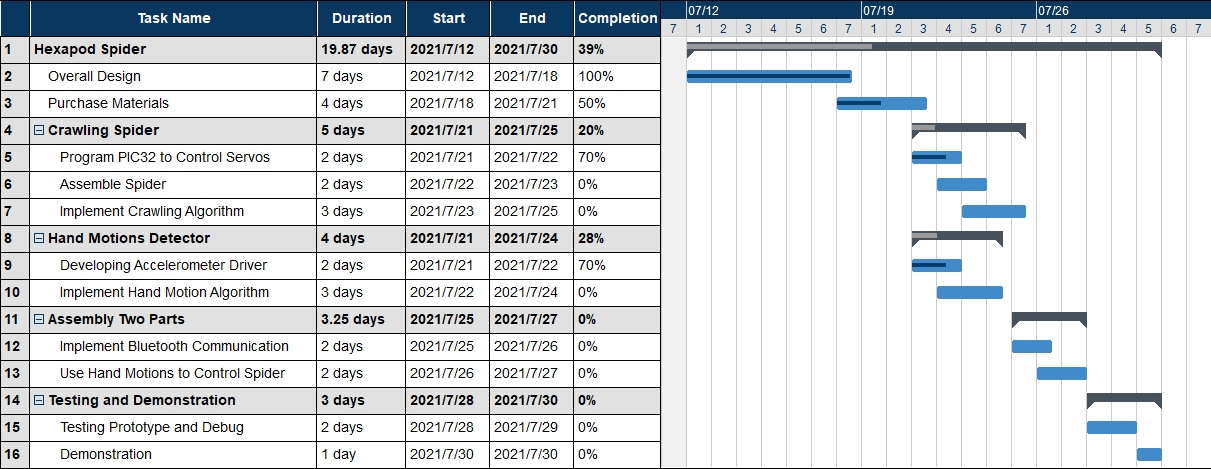
\includegraphics[width=1\textwidth]{Hexapod Spider.jpg}
    \caption{Gantt Chart for developing the Hexapod Spider.}
\end{figure}

The timeline of our final project is shown in Figure 1. We have completed the design part and purchased the materials listed in the previous section. After all the materials are in place, it is expected that on July 21st, we will start developing the Hexapod Spider. The work is divided into two parts, one is the crawling spider and the other is the hand motions detector, and they will start simultaneously. In the crawling spider part, we will spend about two days programming the PIC32 to control servos, two days assembling the spider, and three days implementing and testing the crawling algorithm. In the Hand Motions Detector part, we will spend two days developing the driver for the accelerometer, and three days implementing the hand motion algorithm. After these two parts are finished, we will spend two days making them work together. Then we will spend three days on testing and debugging to ensure there are no serious errors, and prepare the videos and pictures for the final demonstration. 

Hopefully, we can complete these tasks before July 31st, which leaves us three days to deal with unexpected situations and add some extra functions like the distance detector as described in the previous section.

\end{document}